% This LaTeX template is intended for the students of CSI Master from
% University of Bordeaux to make their reports.
%
% This template can be used and modified with no restriction.
%
% %%% History %%%
%
% * April 22, 2014: First version (Emmanuel Fleury <fleury@labri.fr>)
%
% %%% Tips and Tricks %%%
%
% --- The memoir LaTeX class ---
% This template use the 'memoir' class, for more information about
% customization of this class see: http://www.ctan.org/pkg/memoir
%
% --- Rubber ---
% The Makefile are using the Rubber tool, install the 'rubber' package
% to use it properly.
%
\documentclass{backend}

%%%%% Document %%%%%
%%%%%%%%%%%%%%%%%%%%
\begin{document}

\frontmatter%%%%%%%%%%%%%%%%%%%%%%%%%%%%%%%%%%%%%%%%%%%%%%%%%%%%%%%%%%%%
\maketitle
\thispagestyle{empty}

\input{chapters/declaration}

\justifying


\afterpage{%
\vspace{10cm}
\begin{figure*}
    \begin{adjustwidth}{-30mm}{0cm}
        \fbox{\includegraphics[width=0.9\paperwidth]{pictures/page_garde.jpeg}}
    \end{adjustwidth}
    \caption*{\large Art des Spires et plongée Oniriques, \textit{\small{2025}}}
\end{figure*}
}
\chapter*{Résumé}


Ce travail de recherche s'inscrit dans le cadre du développement de la sécurité face aux attaques par canaux auxiliaires, plus précisément une sous-classe : les attaques temporelles. Cette classe d'attaque nécessite seulement l'usage d'un chronomètre pour être mise en œuvre. Cette facilité d'utilisation a rendu les concepteurs de systèmes sécurisés, notamment de bibliothèques cryptographiques, sensibles à ce type de menace et a permis le développement de contre-mesures. De récents travaux ont malheureusement mis en évidence qu'un code source résistant à ce type d'attaque pouvait redevenir vulnérable si compilé avec un mauvais compilateur. Nous allons présenter un outil permettant d'automatiser la vérification de binaires et ainsi d'attester de la sécurité concrète d'une bibliothèque cryptographique. Pour atteindre cet objectif, nous avons conçu un outil de génération de tests permettant une analyse complète de la bibliothèque étudiée. Nous avons aussi développé un ensemble de protocoles permettant de détailler notre méthodologie et d'effectuer une analyse généralisée à plusieurs architectures et à différents compilateurs.

\bigbreak

\textbf{Mots-clés :} Attaque par canal auxiliaire, temps constant, analyse symbolique, vérification formelle, sécurité binaire, compilateurs


\cleardoublepage
\tableofcontents

\newpage\null\thispagestyle{empty}\newpage
\renewcommand\listoflistingscaption{Table des codes}
\listoffigures
\listoflistings
\addcontentsline{toc}{chapter}{Table des codes}
\listoftables

\newpage\null\thispagestyle{empty}
\printindex


\cleardoublepage
\afterpage{%
    \AddToShipoutPictureBG*{%
    \put(2cm,18cm){
        \fbox{\includegraphics[trim = 0cm 16cm 23cm 0cm, clip, scale = 0.4]{pictures/page_garde.jpeg}}}
    }
    \ClearShipoutPicture%
}
\part{Introduction}

\chapter*{Introduction}
\label{chap:introduction}

Le développement sécurisé est une tâche ardue. Si on porte notre regard vers le langage de programmation C, un guide \cite{progC_guide}\footnote{Développé par Anne Canteaut, chercheuse de l'équipe COSMIQ, récemment entrée à l'Académie des Sciences} porté par l'\indexed{INRIA}\footnote{Institut National de Recherche en Informatique et Automatisme} est complet en 133 pages tandis qu'un guide pour du développement sécurisé\cite{anssi_guideForSecureprogramming} produit par l'\indexed{ANSSI}\footnote{Agence nationale de la Sécurité des Systèmes d'Information} comprends 182 pages. Cette comparaison met en évidence la discipline requise par le développeur pour faire de la programmation sécurisée; en sus des connaissances, pour améliorer son efficacité, en cryptologie, en architecture matérielle et en programmation bas niveau .\medbreak

Malheureusement, malgré ces compétences, des erreurs peuvent être produites puis exploiter pour réaliser des attaques sur ces sytèmes sécurisés. Il existe de nombreuses classe d'attaques, certaines exploitant les défauts de conception (type A) tandis que d'autres utilisent les caractéristiques matériels (type B). Pour limiter ces effets de bords, la pratique de la programmation formelle permet de contraindre le développeur et empêcher l'apparitions de ces erreurs. La production de preuve formelle du code à l'issu de cet exercice permet d'avoir des garanties contres les attaques de type A.

En revanche, pour se défendre d'attaques de type B (ou attaques par canal auxiliaire) dépendantes du matériel support du programme, il est plus difficile d'avoir une méthode miracle. Actuellement, la solution la plus courante est d'identifier les attaques existantes pour ajouter les contre-mesures adéquates permettant d'avoir un système sécurisé. Une sous-classe d'attaque continue malgré tout de résister à cette méthode : les attaques temporelles.\medbreak

Découverte par Paul Kocher en 1996 \cite{crypto-1996-1469}, il les décrit comme <<\textit{une mesure précise du temps requis par des opérations sur les clées secrètes, permettrait à un attaquant de casser le cryptosystème}>>. Face à cette menace, l'enjeu d'avoir un code \textit{\indexed{achrognostique}}\footnote{Néologisme de Thomas Pornin dans son article \textit{Constant-Time Code: The Pessimist Case} \cite{constantTimePornin} pour désigner un code sans connaissance de temps} vient se rajouter aux pratiques de programmations sécurisées. Et pourtant, si contre les attaques de type A on arrive à concevoir des preuves mathématiques de sécurité associées à nos systèmes sécurisés, les garanties contre les attaques de type B sont plus faible ou inexistente.\medbreak

En 2024, les travaux de \citeauthor{schneider2024breakingbadcompilersbreak} \cite{schneider2024breakingbadcompilersbreak} prouvent qu'un usage inadapté de compilateur sur un système sécurisé introdui des failles exploitables. Ces résultats, observables partiellement avec des travaux antérieurs (par exemple \cite{binsecRel2019}), montrent qu'un usage inadéquat d'options fournies au compilateur optimise un code prouvé sécurisé et retire les protections indiquées par le développeur. Cela nous amène à plusieurs questions de recherche (QR) que nous tenterons de répondre à travers ce document.
\begin{enumerate}
    \item[\textbf{QR1}] Est-il possible de détecter les failles qui permettent une attaque temporelles ?
    \item[\textbf{QR2}] Est-il possible d'automatiser la détection de ces failles ?
    \item[\textbf{QR3}] Est-il possible d'étendre ce méchanisme entre différentes architectures ?
\end{enumerate}

Les réponses à ces questions permettraient de développer des systèmes sécurisés, communs entre différents supports et d'avoir des garanties de sécurité.

\begin{Acorriger}{Fin d'introduction - à finir}
    Dans la première section nous reviendrons sur les attaques temporelles, leurs impacts et comment s'en protéger. Puis, Dans la deuxième section nous présenterons les outils disponibles à l'analyse et pour la détection de failles. Nous continuerons, dans la troisième section, avec la présentation de nos contributions. \textit{Enfin, dans la quatrième section nous présenterons les mécanismes présent au plus bas niveau de l'informatique pour se protéger des attaques temporelles.}\medbreak
    Ce travail a été réalisé au sein du centre INRIA de Paris dans le cadre du projet \textit{Everest} concernant la mise au point de Hacl*.
    
\end{Acorriger}

\addcontentsline{toc}{chapter}{Introduction}
\chapter*{Projets supports}
\label{chap:supports}

Nous présentons succinctement les deux projets servant de fondations à la réalisation des travaux présentés dans ce mémoire.

\subsection*{\indexed{HACL*}}
Acronyme pour "High assurance cryptography library"\footnote{\url{https://hacl-star.github.io/}}, lire \textit{"HACL star"}. Il s'agit d'une bibliothèque cryptographique développée au sein du \textbf{\indexed{Projet Everest}}\footnote{\url{https://project-everest.github.io/}}. Initié en 2016, ce projet porté par des chercheurs de l'Inria (équipe PROSECCO\footnote{Équipe de recherche rattachée au centre Inria de Paris, focalisée sur les méthodes formelles et la recherche en protocoles cryptologiques. Pour atteindre ces objectifs, l'équipe développe des langages de programmation, des outils de vérification\dots}), du \indexed{Centre de Recherche Microsoft} et de l'\indexed{Université Carnegie Mellon} a pour but de concevoir des systèmes informatiques formellement sécurisés, appliqués à l'environnement HTTPS. Cette bibliothèque, écrite en \indexed{F*} ("F star"), implémente tous les algorithmes de cryptographie modernes et est prouvée mathématiquement sûre. Elle est ensuite transcrite en C pour être directement employée dans n'importe quel projet. HACL* est notamment utilisé dans plusieurs systèmes de production, notamment Mozilla Firefox, le noyau Linux, le VPN WireGuard,\etc.


\subsection*{\indexed{Binsec}}
Binsec (contraction de \textit{Binary Security})\footnote{\url{https://binsec.github.io/}} est une plateforme open source développé pour évaluer la sécurité des logiciels au niveau binaire. Ce logiciel est développé et maintenu par une équipe du CEA List de l'\indexed{Université Paris-Saclay}, et accompagné de chercheurs de \indexed{Verimag}\footnote{Verimag est un laboratoire spécialisé dans les méthodes formelles pour une informatique sûre, avec des applications aux systèmes cyber-physiques. Fondé en 1993 au sein de l'Université Grenoble Alpes, puis rejoint par le CNRS, il a pour objectif la sécurité informatique dans les domaines des transports et de la santé.} et du \indexed{LORIA}\footnote{Laboratoire lorrain de recherche en informatique et ses applications; créé en 1997, c'est un centre de recherche commun au CNRS, à l'Université de Lorraine, à CentraleSupélec et à l'Inria.}. Il notamment est utilisé pour la recherche de vulnérabilités, la désobfuscation de logiciels malveillants et la vérification formelle de code binaire. Grâce à l'exécution symbolique Binsec peut explorer et modéliser le comportement d'un programme pour détecter des erreurs; détection réalisée en association avec des outils de fuzzing et/ou des solveurs SMT.

\addcontentsline{toc}{chapter}{Préambule}

\mainmatter%%%%%%%%%%%%%%%%%%%%%%%%%%%%%%%%%%%%%%%%%%%%%%%%%%%%%%%%%%%%%
\afterpage{%
    \AddToShipoutPictureBG*{%
    \put(0.25\paperwidth,4cm){
        \fbox{\includegraphics[trim = 16cm 0cm 0cm 23cm, clip, scale = 0.5]{pictures/page_garde.jpeg}}}
    }
    \ClearShipoutPicture%
}
\part{\textit{Constant time} : implémentation et vérification}

\chapter{Présentation, enjeux et attaques}
\label{chap:constantTimePresentation}


Ce premier chapitre a pour but de présenter les enjeux de la sécurité informatique face aux attaques par canal auxiliaire et d'introduire les attaques temporelles. Nous distinguerons ces attaques en deux catégories, montrant ainsi la diversité et les potentiels dangers pour un système sécurisé ignorant de cette menace.



\section{L'exécution du code est observable...}

L'Informatique repose sur deux fondations que nous tendons à distinguer dans l'enseignement : le matériel et le logiciel. Pourtant, si nous gardions séparé ces deux domaines, nous aurions des tas de piles de métal et de plastiques d'un côté et des bibliothèques pleines d'idées intéressantes de l'autre. Au contraire, combiner les deux parties permet de réaliser des prouesses technologiques et scientifiques. Ainsi, lorsque nous concevons un système sécurisé, il nous faut prendre en compte ces deux composantes. Pour implémenter un système sécurisé, il ne faut pas seulement avoir un logiciel sécurisé, il est tout aussi important d'avoir un support physique sécurisé. Oublier ce détail, c'est oublier que programmer peut se résumer à manipuler de l'électricité.\medbreak

Les attaques par canal auxiliaires consistent à exploiter les caractéristiques matériels du support pour gagner en connaissances sur un programme ciblé. Puis exploiter ces connaissances pour acquérir d'avantages d'informations privées : identifiants, clés secrètes, messages personnels. Nous leurs attribuons le terme "canal auxiliaire" car il ne s'agit pas de trouver une faille perdue dans les limites d'un logiciel ou d'exploiter une mécanique du logiciel pour sortir de l'espace prévu par le concepteur. Il s'agit de se positionner hors du cadre de développement. Voici quelques travaux présentant une attaque par canal auxiliaire et le canal exploité:
\begin{itemize}
    \item[\cite{DPA_Attack}] Consommation d'énergie 
    \item[\cite{Branch_Attack}] Prédiction de branchement 
    \item[\cite{Thermal_Attack}] Variation de température
    \item[\cite{DRAM_Attack}] Accès à la mémoire DRAM
\end{itemize}\medbreak

Le point commun entre ces attaques est la nécessité d'avoir un point de contact avec la cible. Il faut que l'attaquant puisse récupérer le matériel informatique ou le programme qu'il souhaite attaquer pour ensuite poser des sondes/capteurs afin d'accumuler de la connaissance et monter son exploitation.\bigbreak


Une autre technique d'attaque consiste à venir introduire une erreur dans le déroulement normal d'un programme. Il s'agit d'une attaque par injection de faute. Originellement \cite{faultOverview} les fautes étaient "naturelles" : un défaut dans le code, un problème avec la transcription vers du code machine, un défaut d'un composant dans le système ou une interférence. Ces interférences sont causées par une irrégularité de l'alimentation électrique, des radiations électromagnétiques, une perturbation environnementale \etc\dots
En 2004, \citeauthor{Fault_Attacks} dans leur article \citetitle{Fault_Attacks} \cite{Fault_Attacks} effectuent un tour d'horizon des techniques, montrant l'efficacité de cette méthode sur \indexed{RSA}
% \footnote{Chiffrement asymétrique par clés secrètes du nom de ces auteurs. Standardisé en 1983.}
, \indexed{NVM}\footnote{Non Volatile Memory ou mémoire non volatile est un composant informatique qui conserve son contenu en l'absence d'électricité.}
, \indexed{DES}%\footnote{Algorithme de chiffrement symétrique par bloc. Standardisé en 1977}
, \indexed{EEPROM}\footnote{Electrically-Erasable Programmable Read-Only Memory ou mémoire morte effaçable électriquement et programmable.}, \indexed{JVM}\footnote{Machine virtuelle qui exécute des programmes compilés en bytecode Java.}. Nous retrouvons enfin une liste de contre-mesures et de méthodes de protection contre ces attaques.\medbreak

Ainsi, donner un accès physique à un inconnu est une porte d'entrée pour un attaquant. Pourtant, penser que l'accès physique au support est une condition nécessaire et suffisante pour réaliser une attaque par canal auxiliaire est une erreur.

\section{...à distance}

En effet, il est possible de réaliser des attaques à distance en exploitant d'autres failles de sécurité d'un programme ou d'autres caractéristiques matériels. L'attaque présentée par \citeauthor{LLC_attack} dans \citetitle{LLC_attack} \cite{LLC_attack} repose sur la conception des services clouds où les machines virtuelles accèdent au même matériel. Tandis que la virtualisation crée l'illusion de compartimentation entre les sessions, en réalité, les adresses mémoire pointent vers une ressource physique partagée. Ainsi, l'exploitation du cache du dernier niveau (LLC) permet à un co-hôte de récupérer les clés secrètes d'un autre utilisateur. L'attaquant remplit le cache, puis mesure les temps d'accès vers ces registres, si des modifications apparaissent dans ces temps, cela signifie que la victime a accédé à ces registres. En répétant cette opération, l'attaquant peut reconstruire les clés secrètes de la victime.\medbreak


D'autres attaques distantes comme celle de \citeauthor{LLC_attack} existent \cite{cryptoeprint:2016/224,Moghimi_2017,vanbulck2018nemesis}, mais nous observons rapidement que ces techniques emploient aussi la méthode de chronométrage. En effet, si nous ciblons un algorithme et que nous mesurons son temps d'exécution, si en fournissant différentes entrées (considérées secrètes) des variations sont observées entre les mesures, alors cela signifie que l'algorithme présente une dépendance à ces entrées. Une sous-fonction de cet algorithme est généralement responsable de ces variations. Cette classe d'attaque est appelée <<\textit{attaque temporelle}>>\footnote{Le terme générique dans la recherche scientifique est <<\textit{time attack}>>. Une traduction plus précise serait <<\textit{attaque par chronométrage}>>. Nous choisissons ici d'utiliser le terme <<\textit{attaque temporelle}>> car il est moins lourd et renvoie directement vers la faille exploitée plutôt que par la méthode employée.}.\medbreak

Le lien entre temps et exécution de code est connu depuis le début de l'informatique. Le temps est le marqueur de performance, d'efficacité d'un programme. En revanche, l'idée d'exploiter cet indice pour réaliser une attaque est arrivée plus tardivement. \citeauthor{crypto-1996-1469} nous présente, le premier en 1996, comment monter une attaque en utilisant ce canal.\medbreak

Ce lien entre le temps et l'exécution du code est connu, pourtant la mesure de l'ampleur de la fuite d'information transmise par ce canal n'est pas triviale, ni à son époque, ni aujourd'hui.

\begin{listing}[!ht]
    \caption{Exemple de code vulnérable à une attaque temporelle}
    \label{lst:timing_attack_example}
    \begin{minted}[frame=lines,framesep=2mm,baselinestretch=1.2,fontsize=\footnotesize,linenos, gobble=6]{C}
        bool check_pwd(msg, pwd){
        if (msg.length != pwd.length){
            return False
        }
        for(int i = 0; i < msg.length; i++){
            if(msg[i] != pwd[i]){
            return False
            }
        }
        return True
        }
    \end{minted}
\end{listing}
                
Si nous prenons le code présenté par le code \ref{lst:timing_attack_example}, nous pouvons observer que la fonction \texttt{check\_pwd} compare deux chaînes de caractères. Si elles sont de même longueur, elle les compare caractère par caractère. Si elles sont de longueur différentes, la fonction retourne immédiatement \texttt{False}. Ainsi, si nous fournissons un mot de passe de longueur différente, le temps d'exécution sera constant et court. En revanche, si nous fournissons un mot de passe de même longueur, le temps d'exécution dépendra du nombre de caractères identiques consécutifs entre les deux chaînes. En effet, la fonction s'arrêtera dès qu'un caractère différent est trouvé. Ainsi, en mesurant le temps d'exécution pour différents mots de passe, un attaquant peut déduire des informations sur le mot de passe correct.\medbreak

Nous pouvons synthétiser les exécutions de la fonction \texttt{check\_pwd} en un graphe comme celui présenté par la figure \ref{fig:timing_attack_example}. Chaque interruption de la fonction peut être observée et mesurée, permettant ainsi de régénérer le mot de passe. Bien sûr, la connaissance du protocole ciblé est requise, ou alors il faut réaliser un travail de rétro-ingénierie pour calibrer l'attaque.\medbreak

\begin{figure}[!ht]
    \caption{Suivi du temps d'exécution pour différents mots de passe}
    \label{fig:timing_attack_example}
    \center
    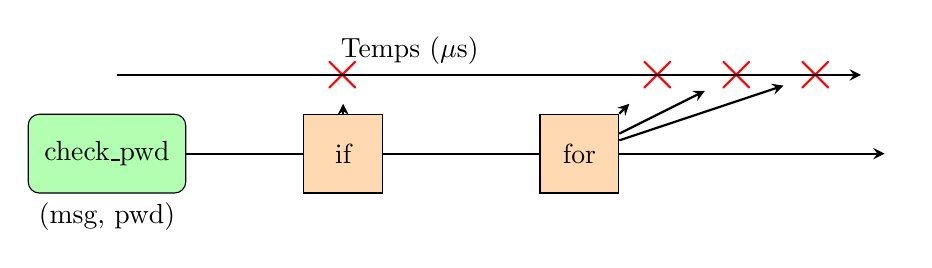
\begin{tikzpicture}[auto]

    % Styles
    \tikzstyle{startstop} = [rectangle, rounded corners, minimum width=2cm, minimum height=1cm, text centered, draw=black, fill=green!30]
    \tikzstyle{process} = [rectangle, minimum width=1cm, minimum height=1cm, text centered, draw=black, fill=orange!30]
    \tikzstyle{arrow} = [thick,->,>=stealth]
    \tikzstyle{arrowred} = [thick,->,>=stealth, draw=red]
    
    % Noeuds
    \node (start) [startstop] {check\_pwd};
    \node (valid) [right of=start, xshift=9cm, green] {\huge{$\checkmark$}};
    \draw [arrow] (start) -- (valid);
    
    \node (inputs) [below of = start, yshift=0.2cm] {(msg, pwd)};
    \node (if) [process] [right of=start, xshift=2cm] {if};
    \node (not) [above of=if, red] {\huge{$\times$}};
    \node (for) [process] [right of=if,, xshift=2cm] {for};
    \node (for1) [above of=for,xshift=1cm, red] {\huge{$\times$}};
    \node (for2) [right of=for1, red] {\huge{$\times$}};
    \node (for3) [right of=for2, red] {\huge{$\times$}};

    \draw [arrow] (if) -- (not);
    \draw [arrow] (for) -- (for1);
    \draw [arrow] (for) -- (for2);
    \draw [arrow] (for) -- (for3);

    \node (t) [above of=start] {};
    \node (a) [above of=valid, xshift=-0.3cm] {};
    \draw [arrow] (t) -- node[above left] {Temps ($\mu$s)} (a.west);
    
    \end{tikzpicture}
\end{figure}

Cette méthode est plus efficace qu'une attaque par force brute. En effet, si le mot de passe est composé de 8 caractères de l'alphabet latin, alors il y a 256 possibilités par caractère, pour un total de $256^8 = 2^{64}$ possibilités. En revanche, si nous utilisons la méthode de l'attaque temporelle, le nombre de possibilités est réduit à $8 + 8 \times 256 = 2056$ possibilités. En effet, nous cherchons dans un premier temps à identifier la longueur du mot de passe, puis nous identifions ensuite caractère après caractère pour trouver le mot de passe. Des temps d'exécution courts correspondent à des cas d'échec, tandis qu'un allongement du temps d'exécution nous permet de déterminer une bonne piste.\medbreak

Les attaques temporelles présentent la particularité d'être génériques. Tandis que les attaques décrites précédemment nécessitent des conditions d'accès ou d'initialisation plus importantes, cette classe d'attaque présente l'avantage d'être réalisable sur tous les types de systèmes, et notamment les systèmes accessibles par internet. La connaissance de cette menace est donc primordiale pour l'implémentation et la mise en service de produits sur Internet.\medbreak

Par la suite du document, le terme "fuite" sera utilisé pour désigner un extrait du programme qui peut être exploité pour réaliser une attaque temporelle. Si nous reprenons le code \ref{lst:timing_attack_example}, les branchements conditionnels lignes [4, 6] sont des fuites d'informations. C'est grâce à ces instructions que l'attaque décrite précédemment est réalisable.\medbreak

\raggedbottom
\textit{Nous allons maintenant nous intéresser aux moyens et méthodes à notre disposition pour se protéger contre les attaques temporelles.}




\chapter{Protection}
\label{chap:constantTimeSolution}

Ce deuxième chapitre montre les innovations nécessaires pour se protéger des attaques temporelles. Nous y découvrons les bonnes pratiques de programmation, les premiers outils automatiques de vérification de code ainsi que les limitations auxquelles est confronté le développeur qui souhaite être résistant à ces attaques.


\section{Bonnes pratiques et usages}

Face à la menace des attaques temporelles, quelles solutions peuvent être mises en place pour protéger nos systèmes informatiques ? Cette attaque a besoin d'un accès au système et d'un chronomètre. Comme nous sommes dans un contexte de systèmes accessibles par internet, altérer ou retirer l'accès signifie perdre en qualité ou supprimer le service proposé. Il faut donc que notre approche cible plutôt l'utilisation du chronomètre.

Il faut donc programmer de telle sorte que sur toutes les entrées possibles de notre système informatique aucune variation de temps ne peut être observée entre les exécutions.
Trois méthodes existent pour pallier ce problème.\medbreak

\subsection*{Programmation en temps constant}
La programmation en temps constant ou <<\textit{Constant-Time Programming}>>, est une pratique de programmation qui vise à résoudre exactement ce problème. Directement lié à la complexité algorithmique, cette pratique modifie et adapte les algorithmes pour que toutes les opérations effectuées aient un temps d'exécution identique.

\citeauthor{BearSSL} \cite{BearSSL} présente tous les éléments à adapter pour configurer un code respectant la politique de programmation en temps constant. Si les opérations élémentaires respectent "naturellement" cette politique; les \textbf{accès mémoires}, les \textbf{sauts conditionnels}, les \textbf{opérations de décalages/rotations} et les \textbf{divisions/multiplications} sont les opérations à adapter en fonction de la plateforme cible. Les descriptions rapportées ci-dessous sont issues de \cite{BearSSL}.\smallbreak

\begin{CitationBox}{Accès mémoire}
  Un chargement depuis la mémoire d'une information est une source de variation. Nous avons vu précedemment \cite{LLC_attack,DRAM_Attack} que l'usage d'un cache mémoire est un canal d'accès pour réaliser une attaque. En effet, l'utilisation d'un cache permet de distinguer les appels entre les données déjà mises en mémoire ou pas. De plus, les changements de valeur dans celui-ci peuvent aussi être observés après exécution.
\end{CitationBox}
\vspace{0.1cm}
\begin{CitationBox}{Décalage et rotation}
  Ces opérations binaires sont ou ne sont pas en temps constant en fonction des CPU sur lesquels le code est exécuté. Certains ont un "barrel shifter" qui permet d'effectuer directement les instructions correspondantes. Cela impacte directement les algorithmes dépendants de décalages logiques comme le chiffrement RC5.
\end{CitationBox}
\vspace{0.1cm}
\begin{CitationBox}{Saut conditionnel}
  Les saut conditionnels sont des instructions qui, comme pour les accès mémoire, demandent de charger les adresses des instructions suivantes. Or, comme un compilateur tend à précharger les instructions suivantes, il va charger les deux côtés du saut conditionnel puis défausser la branche inutile; ce qui entraîne un léger ralentissement. En revanche, il est important de noter que si le branchement est indépendant d'une variable secrète, il n'est pas nécessaire de le modifier. Par exemple si j'ai un compteur et que mon programme doit terminer après un certain nombre d'itérations, aucune fuite ne sera observée.
\end{CitationBox}
\vspace{0.1cm}
\begin{CitationBox}{Division}
  Certaines architectures ont des instructions de divisions spécifiques qui permettent d'accélérer le calcul, les autres emploient des sous-programmes dédiées souvent optimisés en opération de masquage et de décalage. La norme C entraîne elle aussi de la confusion car elle impose $(-1)/2 = 0$; il faut donc être familier avec les spécificités du processeur pour affiner l'usage de cette opération.
\end{CitationBox}
\vspace{0.1cm}
\begin{CitationBox}{Multiplication}
  Enfin, la multiplication, elle aussi dépendante des variables d'entrées, présente une fuite d'information importante. Mais les CPU les plus récents (rédigé en 2016) ont implémenté cette opération en temps constant. Cela suit l'évolution des compilateurs et des processeurs qui tendent à accélérer les opérations et réduire le nombre d'instructions total.
\end{CitationBox}
\vspace{0.1cm}

En reprenant ces règles, nous pouvons modifier notre exemple de code \ref{lst:timing_attack_example} et appliquer des modifications sur les lignes que nous avons déjà ciblées comme fuites d'informations. Les modifications sont libres au choix du concepteur. Voici une correction qui peut être réalisée :

\begin{listing}[!htb]
    \caption{Exemple de correction pour rendre un code résistant aux attaques temporelles}
    \label{lst:timing_attack_CT_example}
    \begin{minted}[frame=lines,framesep=2mm,baselinestretch=1.2,fontsize=\footnotesize,linenos, gobble=6]{C}
        bool check_pwd(msg,pwd) {
          // Hachage
            char msg_hash[SHA256_DIGEST_LENGTH]; sha256_hash_string(msg, msg_hash);
            char pwd_hash[SHA256_DIGEST_LENGTH]; sha256_hash_string(pwd, pwd_hash);

            // Comparaison
            bool equal = true;
            for (int i = 0; i < SHA256_DIGEST_LENGTH; i++) {
                equal &= msg[i] != pwd[i]
            }
            return equal;
        }
    \end{minted}
\end{listing}

Nous voyons que le premier branchement a été remplacé par un hachage des paramètres d'entrées. Cette opération est considérée ici en temps constant mais peut ne pas l'être. Il faut être vigilant sur toutes les briques d'algorithme que nous souhaitons utiliser. Enfin, le second branchement conditionnel est purement supprimé, le parcours des tableaux se fait entièrement.\bigbreak

Avec cette modification, nous avons un code \ref{lst:timing_attack_CT_example} qui ne présente plus de fuite de données. Pourtant, nous pouvons avoir un doute sur l'usage de la fonction "\textit{sha256\_hash\_string}". Si cette fonction n'est pas elle même implémentée selon la politique temps constant, nous avons alors introduit une nouvelle surface de fuite d'informations. Il faut vérifier notre code pour supprimer ce doute.\medbreak

\subsection*{Outils de garanties}

Plusieurs outils existent et peuvent être utilisés tous au long du processus de développement d'un système sécurisé. Cela peut être durant la phase de conception du code source, au moment de la compilation ou encore en vérification de la compilation.\smallbreak


Une solution légère est de ce servir du système libre <<\textbf{Compiler Explorer}\footnote{\url{https://godbolt.org/}}>>. Avec à disposition un éditeur de texte, il est possible de voir comment sera généré le code assembleur. En reprenant une partie du code \ref{fig:timing_attack_example}, nous pouvons voir sur la figure \ref{img:godbolt_example} que le choix du compilateur, ici sa version, introduit une légère modification. Ce changement n'est pas perceptible sans observation directe, il se perçoit directement grâce à la petite taille du code observé. Un autre exemple \ref{fig:comparaison_assembleur} est présenté à la fin du chapitre.

\begin{figure}[!h]
  \begin{adjustwidth}{-18mm}{0mm}
    \centering
    \includegraphics[trim = 1mm 0mm 0mm 0mm, clip,width=0.9\paperwidth]{pictures/godbolt_example.png}
    \caption{Capture d'écran de comparaison de code assembleur x86\_64 entre \texttt{GCC 5.1} et \texttt{GCC 15.1}}
    \label{img:godbolt_example}
  \end{adjustwidth}
\end{figure}

Si nous souhaitons faire une analyse à l'échelle d'un projet, ce parcours à la main des fonctions ou de morceaux de fonctions est réellement fastidieux. Il faut mieux déléguer ce travail à un outil conçu pour vérifier la présence de fuite.\smallbreak

Plusieurs articles référencent l'ensemble des outils existants \cite{notThatHardCT, GeimerEvaluationsSideChannel} pour réaliser ce travail. Le tableau \ref{tab:tools_ct} de \citeauthor{notThatHardCT} liste 24 outils en libre accès conçus pour détecter des failles par canal auxiliaire.

Ils sont listés alphabétiquement et ont précisé le type de fichier analysé (\textit{Cible}), la méthode d'analyse réalisée (\textit{Techn.}) et les garanties attendues de ces analyses (\textit{Garanties}). Nous reviendrons plus en détail sur ces méthodes et leurs fonctionnements dans le chapitre \ref{chap:automateVerifOutils}.\medbreak

\begin{table}[!ht]
  \caption{Liste d'outils de vérification, source \cite{notThatHardCT} }
  \label{tab:tools_ct}
  \scriptsize{
  Cible : [C, Java] = Code source, Binaire = Binaire, DSL = Surcouche de langage, Trace = Trace d'exécution, WASM = Assembleur web.\\
  Techn. : Formel = Programmation formelle, [Symbolique, Dynamique, Statistique] = type d'analyse. \\
  Garanties (\textit{Sécurité face aux attaques temporelles}) : $\bullet$ = Analyse correcte, $\blacktriangle$ = Correcte mais avec des limitations, $\circ$ = Aucune garantie, $\bigstar$ = Vérification d'autres propriétés.
  }
  \normalsize
  \begin{center}
    \begin{tabular}{lccc}
    \hlineB{2}
    \textbf{Outil} & \textbf{Cible} & \textbf{Techn.} & \textbf{Garanties} \\
    \rowcolor{lightgray}
    ABPV13 \cite{ABPV13} & C & Formel & $\bullet$ \\
    Binsec/Rel \cite{binsecRel2019} & Binaire & Symbolique & $\blacktriangle$ \\
    \rowcolor{lightgray}
    Blazer \cite{Blazer} & Java & Formel & $\bullet$ \\
    BPT17 \cite{BPT17} & C & Symbolique & $\blacktriangle$ \\
    \rowcolor{lightgray}
    CacheAudit \cite{CacheAudit} & Binaire & Formel & $\bigstar$ \\
    CacheD \cite{CacheD} & Trace & Symbolique & $\circ $ \\
    \rowcolor{lightgray}
    COCO-CHANNEL \cite{COCOCHANNEL} & Java & Symbolique & $\bullet$ \\
    ctgrind \cite{ctgrind} & Binaire & Dynamique & $\blacktriangle$ \\
    \rowcolor{lightgray}
    ct-fuzz \cite{ctfuzz} & LLVM & Dynamique & $\circ$ \\
    ct-verif \cite{ctverif} & LLVM & Formel & $\bullet$ \\
    \rowcolor{lightgray}
    CT-WASM \cite{CTWASM} & WASM & Formel & $\bullet$ \\
    DATA \cite{DATA1,DATA2} & Binaire & Dynamique & $\blacktriangle$ \\
    \rowcolor{lightgray}
    dudect \cite{dudect} & Binaire & Statistique & $\circ $ \\
    FaCT \cite{FaCT} & DSL & Formel & $\bullet$ \\
    \rowcolor{lightgray}
    FlowTracker \cite{FlowTracker} & LLVM & Formel & $\bullet$ \\
    haybale-pitchfork \cite{haybale-pitchfork} & LLVM & Symbolique & $\blacktriangle$ \\
    \rowcolor{lightgray}
    KMO12 \cite{KMO12} & Binaire & Formel & $\bigstar$ \\
    MemSan \cite{MemSan} & LLVM & Dynamique & $\blacktriangle$ \\
    \rowcolor{lightgray}
    MicroWalk \cite{MicroWalk} & Binaire & Dynamique & $\blacktriangle$ \\
    SC-Eliminator \cite{SCEliminator} & LLVM & Formel & $\bullet$ \\
    \rowcolor{lightgray}
    SideTrail \cite{SideTrail} & LLVM & Formel & $\bigstar$ \\
    Themis \cite{Themis} & Java & Formel & $\bullet$ \\
    \rowcolor{lightgray}
    timecop \cite{timecop} & Binaire & Dynamique & $\blacktriangle$ \\
    VirtualCert \cite{VirtualCert} & x86 & Formel & $\bullet$ \\
    \hlineB{2}
    \end{tabular}
  \end{center}
\end{table}

\newpage
Une dernière solution serait d'utiliser un compilateur spécialisé qui produit un code assembleur sans fuite \cite{Borrello_2021, Raccoon} ou d'utiliser un compilateur formel comme \textit{CompCert} \cite{compcert-CT}. Cette solution rencontre en pratique de nombreux problèmes que nous conservons pour la section \ref{sect:limitations} \nameref{sect:limitations}.

\subsection*{Écriture en code assembleur}

Enfin, la dernière méthode pour obtenir un code sécurisé et sans fuite c'est de programmer directement en assembleur. De cette manière, nous avons un contrôle total sur le flot d'exécution de notre programme, nous pouvons insérer des optimisations qu'un compilateur pourrait ignorer. Écrire en assembleur requiert de connaître la plupart des opérandes disponibles pour l'architecture ciblée et les modèles des composants présents sur le support. Cela nous amène directement aux limitations induites par cette solution.

\section{Limitations}
\label{sect:limitations}

Écrire en assembleur c'est écrire spécifiquement pour une architecture de processeur. Il faut connaître les instructions adéquates, les potentielles optimisations qui existent sans parler de la syntaxe particulère qui rend son développement plus lent. Travailler en assembleur c'est limiter la portabilité du code proposé. Or l'objectif derrière le développement d'une bibliothèque sécurisée est de pouvoir être employée par le plus de configurations possibles pour se protéger d'attaques.\smallbreak

Face à cette situation, nous pouvons choisir d'utiliser un compilateur spécialisé (\cite{Borrello_2021, Raccoon}). Et comme un serpent qui se mord la queue, nous voici à nouveau limités. Ces compilateurs peuvent ne pas supporter l'ensemble du jeu d'instruction d'une architecture, ils peuvent avoir besoin d'instructions supplémentaires (des annotations de code) pour réaliser leur compilation, ils peuvent ne pas implémenter les optimisations présentent sur les processeurs les plus récents.\smallbreak

Donc, si les compilateurs spécialisés ne sont pas envisageables, nous nous retrouvons à utiliser les compilateurs courants \texttt{GCC} et \texttt{LLVM+Clang} pour notre solution sécurisée. Nous devons donc programmer en respectant la politique temps constant. Et si cette pratique semble être notre solution, nous pouvons lire dans l'article de présentation de l'outil d'analyse Binsec \citetitle{binsecRel2019} : 
\begin{CitationBox}{Conclusion - \cite{binsecRel2019}}
Nous avons découvert que \texttt{gcc -O0} et des optimisations de \texttt{clang} introduisent des infractions à la politique temps constant indétectées par les outils antérieurs
\end{CitationBox}\smallbreak

Cette, annonce discrète au sein du document, a ensuite été prise en compte par \citeauthor{schneider2024breakingbadcompilersbreak} qui a mené une enquête sur les bibliothèques cryptographiques sécurisées et résistantes aux attaques temporelles : \cite{schneider2024breakingbadcompilersbreak}. La conclusion principale est que les compilateurs modernes sont devenus assez performants pour voir à travers les astuces employées et qu'une mauvaise utilisation d'optimisation implique l'introduction de faille de sécurité. \smallbreak

Voici un exemple communiqué par \citeauthor{schneider2024breakingbadcompilersbreak} auprès des chercheurs de HACL*. Nous pouvons voir deux fonctions dans le code \ref{lst:Hacl_masking}, <<\textit{cmovznz4}>> et <<\textit{FStar\_UInt64\_eq\_mask}>>. La première appelle la seconde pour générer un masque qui sera ensuite appliqué aux paramètres de <<\textit{cmovznz4}>>. Nous avons ici une fonction qui agit comme un branchement conditionnel. Si \texttt{cin} vaut 1, alors $r = x$ sinon $r = y$.

\begin{listing}[!ht]
    \caption{Fonction de masquage issu de \textit{HACL*}}
    \label{lst:Hacl_masking}
    \begin{minted}[frame=lines,framesep=2mm,baselinestretch=1.2,fontsize=\footnotesize,linenos]{C}
#include <stdint.h>

static inline uint64_t FStar_UInt64_eq_mask(uint64_t a, uint64_t b)
{
  uint64_t x = a ^ b;
  uint64_t minus_x = ~x + (uint64_t)1U;
  uint64_t x_or_minus_x = x | minus_x;
  uint64_t xnx = x_or_minus_x >> (uint32_t)63U;
  return xnx - (uint64_t)1U;
}

void cmovznz4(uint64_t cin, uint64_t *x, uint64_t *y, uint64_t *r)
{
  uint64_t mask = ~FStar_UInt64_eq_mask(cin, (uint64_t)0U);
  uint64_t r0 = (y[0U] & mask) | (x[0U] & ~mask);
  uint64_t r1 = (y[1U] & mask) | (x[1U] & ~mask);
  uint64_t r2 = (y[2U] & mask) | (x[2U] & ~mask);
  uint64_t r3 = (y[3U] & mask) | (x[3U] & ~mask);
  r[0U] = r0;
  r[1U] = r1;
  r[2U] = r2;
  r[3U] = r3;
}
    \end{minted}
\end{listing}

Avec le compilateur \texttt{RISC-V rv64gc clang 15.0.0}, si nous précisons les options de compilation \texttt{-O0} ou \texttt{-O1}, nous pouvons observer différents résultats. Le plus notable ici est l'apparition de l'instruction \texttt{beqz}, qui est un branchement conditionnel, ainsi que la suppression de la fonction de masquage <<\textit{FStar\_UInt64\_eq\_mask}>>. Les optimisations appelées par l'option \texttt{-O1} identifient le masquage effectué et modifient le code pour accélérer son exécution. L'optimisation \ref{subcode:O0} suit les instructions précisées par le code source, de cette manière le compilateur réalise une compilation rapide. Au contraire de l'optimisation \ref{subcode:O1} qui réalise une analyse plus longue du code source, et donc a une compilation plus lente, mais grâce à l'ajout des branchements successifs (les instructions \texttt{beqz}) permet une exécution plus rapide. Les options de compilation sont indiquées en annexe \ref{tab:compile_option}\footnote{\url{https://gcc.gnu.org/}}.

\begin{figure}[!ht]
    \begin{subfigure}[b]{0.5\textwidth}
        \centering
        \small
        \begin{minted}[frame=single, framesep=2mm, baselinestretch=1.2, fontsize=\footnotesize, linenos]{java}
cmovznz4:
        ...
        li      a1, 0
        call    FStar_UInt64_eq_mask
        not     a0, a0
        sd      a0, -56(s0)
        ld      a0, -40(s0)
        ld      a0, 0(a0)
        ld      a2, -56(s0)
        and     a0, a0, a2
        ld      a1, -32(s0)
        ld      a1, 0(a1)
        not     a2, a2
        and     a1, a1, a2
        or      a0, a0, a1
        sd      a0, -64(s0)
        ...
        ret

FStar_UInt64_eq_mask:
        addi    sp, sp, -64
        sd      ra, 56(sp)
        sd      s0, 48(sp)
        addi    s0, sp, 64
        sd      a0, -24(s0)
        sd      a1, -32(s0)
        ld      a0, -24(s0)
        ld      a1, -32(s0)
        xor     a0, a0, a1
        sd      a0, -40(s0)
        ld      a1, -40(s0)
        li      a0, 0
        sub     a0, a0, a1
        sd      a0, -48(s0)
        ld      a0, -40(s0)
        ld      a1, -48(s0)
        or      a0, a0, a1
        sd      a0, -56(s0)
        ld      a0, -56(s0)
        srli    a0, a0, 63
        sd      a0, -64(s0)
        ld      a0, -64(s0)
        addi    a0, a0, -1
        ld      ra, 56(sp)
        ld      s0, 48(sp)
        addi    sp, sp, 64
        ret
        \end{minted}
        \caption{Option \texttt{-O0}}
        \label{subcode:O0}
    \end{subfigure}%
    ~~
    \begin{subfigure}[b]{0.4\textwidth}
        \centering
        \small
        \begin{minted}[frame=single, framesep=2mm, baselinestretch=1.2, fontsize=\footnotesize, linenos]{java}
cmovznz4:
        mv      a5, a1
        beqz    a0, .LBB0_2
        mv      a5, a2
.LBB0_2:
        beqz    a0, .LBB0_5
        addi    a6, a2, 8
        bnez    a0, .LBB0_6
.LBB0_4:
        addi    a4, a1, 16
        j       .LBB0_7
.LBB0_5:
        addi    a6, a1, 8
        beqz    a0, .LBB0_4
.LBB0_6:
        addi    a4, a2, 16
.LBB0_7:
        ld      a7, 0(a5)
        ld      a5, 0(a6)
        ld      a6, 0(a4)
        beqz    a0, .LBB0_9
        addi    a0, a2, 24
        j       .LBB0_10
.LBB0_9:
        addi    a0, a1, 24
.LBB0_10:
        ld      a0, 0(a0)
        sd      a7, 0(a3)
        sd      a5, 8(a3)
        sd      a6, 16(a3)
        sd      a0, 24(a3)
        ret
        \end{minted}
        \caption{Option \texttt{-O1}}
        \label{subcode:O1}
    \end{subfigure}
    \caption{Comparaison du code \ref{lst:Hacl_masking} en fonction de différentes options de compilation données au compilateur, réalisée avec l'aide de \textit{Compiler Explorer}.}
    \label{fig:comparaison_assembleur}
\end{figure}

\raggedbottom
\textit{Avec ces solutions applicables, il nous faut maintenant étudier leurs impacts. Nous allons voir quels moyens permettent de vérifier la sécurité d'un programme.}

\chapter{Analyse de programmes et méthodes de vérifications}
\label{chap:automateVerifOutils}

Nous allons étudier les moyens à notre disposition pour réaliser une analyse pertinente et efficace d'un programme résistant aux attaques temporelles.

\section{Modélisation d'une attaque}

En sécurité informatique, la première étape, essentielle avant de développer une solution, c'est de produire un modèle du danger contre lequel nous souhaitons nous défendre. On parle parfois de \textit{modèle de fuite}. Cette étape de synthèse et d'abstraction est importante pour identifier les risques encourus par le futur système, souvent en identifiant les points de fuite employés par les attaques déjà publiées. \citeauthor{BewarCTSideChannel} \cite{BewarCTSideChannel} nous donne trois modèles d'adversaires à considérer lorsqu'on souhaite se défendre contre les attaques temporelles :

\begin{table}[!ht]
  \caption{Modèles d'adversaires pour les attaques temporelles \cite{BewarCTSideChannel}}
  \label{tab:temporal_attacks}
  \begin{adjustbox}{width=\textwidth}
  \begin{tabularx}{\textwidth}{|L|L|}
    \hline
    \rowcolor{lightgray}
    \multicolumn{1}{|C|}{\textbf{Type d'attaque}} & \multicolumn{1}{C|}{\textbf{Description}} \\ \hline
    Par chronométrage & Observation du temps de calcul. \\ \hline
    Par accès mémoire & Manipulation et observation des états d'un ou de plusieurs caches mémoire. \\ \hline
    Par récupération de traces & Suivi des appels de fonctions, des accès réussis ou manqués à la mémoire. \\ \hline
  \end{tabularx}
  \end{adjustbox}
\end{table}

Ces types d'attaques forment une base pour la conception de nos modèles d'attaquant. Considérer le mode opératoire <<récupération de traces>> induit un modèle plus puissant. Des travaux comme ceux de \citeauthor{twartingCT} \cite{twartingCT} portent directement sur des améliorations matérielles permettant une défense contre ce modèle. Considérer un hypothétique attaquant plus puissant, avec des accès à des ressources supplémentaires, permet de concevoir un système plus sûr. Certains outils comme \cite{ctfuzz,DATA2} ou cette étude \cite{notThatHardCT} exploitent notamment cette mécanique pour attester de la sécurité d'un programme.\medbreak


Puis, avec ces modèles et les contre-mesures connues, nous pouvons constituer un ensemble de règles qui vérifient ces risques. \cite{CTsaferCrypto} résume celles-ci en une liste de trois règles :
\begin{enumerate}
  \item Toute boucle révèle le nombre d'itérations effectuées. 
  \item Tout accès mémoire révèle l'adresse (ou l'indice) accédée.
  \item Toute instruction conditionnelle révèle quelle branche a été prise.
\end{enumerate}

Avec ces règles, il est alors possible de créer un outil qui analyse les programmes à sécuriser. C'est ainsi que le premier outil existant a été produit : \texttt{ctgrind} (2010).\medbreak

D'autres chercheurs comme \citeauthor{binsecRel2019} \cite{binsecRel2019} s'attellent à la création de modèles formels. Cette méthode demande un travail de formalisation du comportement de programmes binaires et une implémentation plus rigoureuse de leurs outils. Cela permet en retour une évaluation complète et correcte de programmes complexes (\ie primitives cryptographiques asymétriques).

\subsection*{Formalisation de modèle - \cite{binsecRel2019}}

Si nous voulons concevoir un modèle formel, nous pouvons nous appuyer sur l'article \citetitle{formalConstantTime} \cite{formalConstantTime}.\medbreak


Nous commençons par définir un programme. Il s'agit d'une suite d'instructions binaires. Et une instruction est une action sur la mémoire. Cela nous permet de définir notre programme comme une suite de configurations $(l,r,m)$; $l$ la ligne d'instruction, $r$ le dictionnaire de registre et $m$ la mémoire. La configuration initiale est définie par $c_0 \triangleq (l_0,r_0,m_0)$ où $l_0$ est l'adresse de l'instruction d'entrée du programme, $r_0$ un dictionnaire de registres vide et $m_0$ une mémoire vide.\smallbreak

Ainsi, avec cette modélisation, une instruction est un changement appliqué à notre configuration. Ce changement peut être représenté par $ c_0 \underset{t}{\to} c_1 $, $c_0$ et $c_1$ sont deux configurations successives, $\to$ la transition entre les deux et $t$ une fuite émise par cette transition. Notons que certaines instructions ne produisent pas de fuites.\smallbreak

Une fois ce préambule installé nous définissons formellement le comportement de nos instructions. Regardons par exemple comment se formalise un chargement :

\begin{figure}[!ht]
  \caption{Instruction \texttt{chargement}}
  \label{fig:instr_load}
  \centering
  
    % version avec \scalebox
    \scalebox{1.8}{% agrandir à 150%
    $\smash{\scalebox{0.5556}{\textsc{LOAD}}}\quad
    \frac{(l,r,m)\; e \vdash_t \text{bv}}
         {(l,r,m)\; @ \; e \vdash_{t.[\text{bv}]} m \;\text{bv}}$
    }
\end{figure}

Ici, l'évaluation de l'expression \texttt{e} sur une configuration $(l,r,m)$ produit une fuite de la valeur $bv$. En haut nous retrouvons la notation de l'opération effectuée et au-dessous la formalisation de la fuite : $t \cdot [bv]$ signifie que la valeur $bv$ s'ajoute à la liste des fuites. Ce second exemple \ref{fig:instr_branchement} présente une opération de branchement en fonction de $e$ vers les instructions $l_1$ et $l_2$. Nous voyons que la valeur est différente de zéro, ce qui nous produit une fuite vers l'instruction $l_1$. Cette fuite est à ajouter à notre liste $t$.

\begin{figure}[!ht]
  \caption{Instruction \texttt{branchement}}
  \label{fig:instr_branchement}
  \centering
  \scalebox{1.8}{
    $\smash{\scalebox{0.5556}{\textsc{T-ITE}}}\quad
        \frac{
        P.l = \textit{ite } e \,?\, l_1 : l_2 \quad(l, r, m) \vdash_t \text{bv} \quad \text{bv} \neq 0}
        {(l, r, m)\; \underset{t[l_1]}{\longrightarrow}\; (l_1, r, m)}$
    }
\end{figure}

Nous pouvons retrouver l'ensemble des règles formelles en Annexe \ref{fig:ensemble_instr_formelles}.

\section{Analyse d'un programme}

Nous savons concevoir un modèle pour contrôler ou détecter les erreurs. Nous pouvons maintenant concevoir notre analyse pour vérifier ce modèle sur un programme. Plusieurs techniques de vérification existent et nous allons les passer en revue : \cite{GeimerEvaluationsSideChannel}.\medbreak


\subsection*{Analyse statique}

Cette méthode consiste à déduire le fonctionnement d'un programme. Nous souhaitons vérifier que son fonctionnement respecte les propriétés de sécurité définies préalablement. Cette analyse sans exécution réalise une simulation du programme en explorant les chemins d'exécution possibles. De fait, les résultats obtenus sont souvent approximés car une exploration totale peut se révéler irréalisable. Historiquement il s'agit de la première méthode étudiée/employée et depuis elle a été dérivée en plusieurs approches.\medbreak

\paragraph{Non-interférence} Pour renforcer les résultats obtenus et réduire le nombre de faux positifs nous pouvons vérifier la propriété de non-interférence. Cette propriété est inhérente aux programmes. Un programme a des entrées et des sorties. Celles-ci peuvent être classées \textit{faibles} (peu importantes) ou \textit{hautes} (données secrètes, sensibles). Un programme est non-trois modèles d'adversaires à considérer lorsqu'on souhaite se interférent si et seulement si pour n'importe quelle entrée faible le programme ressort la même sortie faible peu importe les valeurs des entrées hautes qui peuvent être précisées.

Appliqué à une analyse statique pour la vérification de programme, la mesure des ressources employées par l'ordinateur permet d'avoir une sortie faible pour comparer le comportement d'un programme en fonction de ses entrées (ici considérées secrètes).

\paragraph{\textit{Self-Composition}}\footnote{Construction personnelle, le terme anglais est conservé.} La self-composition consiste à entrelacer deux exécutions d'un programme $P$ avec différents ensembles de variables secrètes dans un seul programme auto-composé $P;P'$. Des solveurs peuvent alors être utilisés pour vérifier la propriété de non-interférence. Cette approche a été utilisée par \citeauthor{ABPV13} \cite{ABPV13} pour vérifier manuellement des exemples limités, nécessitant de nombreuses annotations pour limiter l'explosion (quadratique) des états à comparer et explorer. \cite{binsecRel2019} emploie cette approche associée à des solveurs SMT pour vérifier uniquement les propriétés définies dans leur modèle. La restriction aux propriétés temps constant permet l'exploitation de cette méthode sans le contrecoup de l'augmentation de la taille des formules.

\paragraph{Systèmes de types} Cette approche diffère des précédentes car elle nécessite un travail supplémentaire du développeur. Il doit ajouter la spécification \texttt{secret} aux valeurs employées pour que cette information se diffuse dans le compilateur et que des mesures adaptées soient effectuées au niveau du binaire. Cette approche est intéressante car elle permet une flexibilité plus importante lors de la production du code et permet de s'abstenir des contre-mesures décrites au chapitre \ref{chap:constantTimeSolution}. En revanche elle nécessite un compilateur spécialisé et aucune vérification sur le binaire produit n'est effectuée. 

\paragraph{Interprétation abstraite} Un programme est (généralement) trop complexe pour être entièrement formellement vérifié, donc il y a une sur-approximation des états atteignables par l'analyse. Ainsi, si l'analyse approximée est sécurisée alors le programme est sécurisé. Cette approche se retrouve dans CacheAudit \cite{CacheAudit} : modélisation par un graphe de flot de l'état des caches, de la mémoire et des successions d'évènements.

\paragraph{Exécution symbolique} L'exécution symbolique consiste à exécuter le programme avec des entrées symboliques. Les chemins explorés sont associés à une formule logique, et un solveur vérifie si un ensemble de valeurs concrètes satisfait les formules générées. Cette méthode est utilisée pour vérifier l'absence de dépendance aux secrets dans les comportements temporels ou mémoire du programme.

\subsection*{Analyse dynamique}

L'analyse dynamique emploie la preuve par l'exemple pour garantir la sécurité du programme cible. Nous exécutons le programme et nous collectons sa trace : informations issues des évènements (accès mémoire, sauts,\etc) rencontrés au fur et à mesure de l'exécution. Les approches diffèrent dans la collecte et la production de ces traces.

\paragraph{Trace unique} Explorer tous les comportements d'un programme est coûteux en temps, et pour les besoins du développement il peut être préférable d'étudier quelques cas particuliers entièrement. Cette approche simplifie le modèle de l'attaquant et réalise sa vérification plus rapidement. \texttt{ctgrind} \cite{ctgrind} réutilise l'analyse dynamique de Valgrind pour vérifier les propriétés temps constant. Pour ajouter de la précision, il est possible d'utiliser l'exécution symbolique pour rejouer la trace avec le secret comme valeur symbolique et vérifier la violation du temps constant (CacheD \cite{CacheD}).

\paragraph{Comparaison de traces} Les tests statistiques peuvent vérifier si différents secrets induisent des différences significatives dans les traces enregistrées. Des outils comme DATA \cite{DATA1} ou MicroWalk \cite{MicroWalk} utilisent diverses méthodes statistiques ou d'apprentissage pour détecter et localiser les fuites. D'autres outils comme dudect \cite{dudect} enregistrent simplement le nombre total de cycles d'horloge et comparent leur distribution selon les secrets.

Le fuzzing peut aussi être utilisé pour trouver des entrées maximisant la couverture et la fuite via canal auxiliaire, comme dans ct-fuzz \cite{ctfuzz}.\medbreak


\section{Outils de vérifications}
% https://blog.cr.yp.to/20240803-clang.html


Nous avons présenté rapidement de nombreux outils capables d'effectuer de la vérification de binaire (voir la table \ref{tab:tools_ct}) et tout au long de la section précédente nous avons présenté les méthodes employées par ceux-ci. \medbreak

Ils sont tous conçus pour analyser spécialement type de fichier (C, Java, LLVM, \etc). Dans notre cas nous ciblons des binaires. Nous pouvons donc nous tourner vers ces candidats :
\begin{itemize}
\begin{multicols}{4}
  \item Binsec
  \item CacheAudit
  \item ctgrind
  \item DATA
  \item dudect
  \item KMO
  \item MicroWalk
  \item timecop
\end{multicols}
\end{itemize}

\subsection*{Outils obsolète ou inadéquat}

\texttt{ctgrind} et \texttt{timecop} sont tous les deux bâtis sur \textit{Valgrind}. L'analyse se base sur l'outil de détection d'erreur mémoire propre à \textit{Valgrind} : \textit{Memcheck}. Celui-ci détecte les branchements conditionnels et les accès mémoire calculés vers des régions non initialisées. Les vulnérabilités sont trouvées en marquant les variables secrètes comme non définies, au travers d'une annotation de code spécifique. Puis, durant l'exécution, \textit{Memcheck} associe chaque bit de données manipulées par le programme avec un bit de définition qu'il propage tout au long de l'analyse et qu'il vérifie lors d'un calcul d'une adresse ou d'un saut. Appliquée à \textit{Valgrind} l'analyse est pertinente. Cependant, dans le cadre de la recherche de failles temporelles cette approche produit un nombre considérable de faux positifs, car des erreurs non liées aux valeurs secrètes sont également rapportées.\medbreak


\texttt{KMO} détecte les fuites d'information pour des attaques qui ciblent le cache. Cet outil développé en 2012 et n'est plus maintenu, utilisait une représentation interne du binaire pour compter les bits d'informations qui peuvent fuiter. En initialisation, l'outil fait deux estimations (borne supérieure et inférieure) de la quantité d'informations qu'un attaquant peut extraire en observant les adresses mémoire présentes dans le cache après l'exécution d'un programme. Grâce à l'observation qu'une estimation haute du nombre d'états atteignables par le programme est aussi une estimation haute du nombre de bits que peut connaître un attaquant, on peut déterminer la sécurité d'un programme.


\subsection*{Outils statistiques}

\texttt{dudect} détecte les fuites temporelles par des mesures répétées du temps d'exécution et une comparaison à l'aide d'un test statistique. Le binaire est exécuté sous deux classes différentes d'entrées secrètes : un ensemble avec des valeurs constantes et un ensemble avec des valeurs sélectionnées aléatoirement avant chaque mesure. Les temps d'exécution de la fonction cible sont alors enregistrés en sondant les compteurs de cycles CPU. Si les deux distributions sont distinguables, alors une fuite est rapportée uniquement si la valeur dépasse un seuil (prédéfini). Les garanties apparaissent à partir d'un grand nombre de mesures.\medbreak

\texttt{MicroWalk} enregistre plusieurs exécutions de la fonction cible avec différentes entrées. La trace enregistrée contient les cibles des branches et les adresses mémoire rencontrées pendant l’exécution. Des scores d’information mutuelle (MI) sont ensuite calculés entre la trace de fuite et l’ensemble des entrées, fournissant une quantification du nombre de bits d’entrée divulgués. \texttt{MicroWalk} propose différents compromis entre granularité du score MI et performance, allant de l’information mutuelle sur l’ensemble du programme (quantification grossière des fuites) jusqu’à des instructions individuelles (pour localiser précisément les fuites).\medbreak

\texttt{DATA} identifie les vulnérabilités par canaux auxiliaires basées sur les adresses grâce à une analyse dynamique. Premièrement, une phase de collecte des traces d’adresses. En comparant ces traces, il identifie des différences au niveau des adresses, indiquant d’éventuelles fuites. Cependant, de nombreuses différences proviennent des entrées publiques et ne sont donc pas critiques. Pour filtrer ces faux positifs, \texttt{DATA} utilise des tests statistiques. La deuxième phase teste si les différences dépendent de la clé privée en comparant des traces générées à partir d’une clé fixe avec des traces générées à partir de clés variables. Ce test entre fixe et aléatoire nécessite un contrôle sur la variable secrète. Enfin il y a une phase de classement des fuites pour détecter les relations entre les traces d’adresses et le secret.\medbreak


\subsection*{Outils formels}


\texttt{CacheAudit} prend en entrée un binaire de programme et une configuration de cache, et il en déduit des garanties de sécurité formelles et quantitatives adaptées à un jeu de modèles d'attaquants par canaux auxiliaires (observation des états de cache, des traces d'utilisation de caches et de chronométrage des temps d’exécution). Le principal défaut est l'usage limité à l'architecture x86\_64.\medbreak


\texttt{Binsec} est une plateforme d'outils. On peut concevoir des scripts ou des extensions pour diriger les analyses qu'il effectue. Il a notamment une extension qui permet d'exploiter l'exécution symbolique pour vérifier les propriétés de temps constant d'un binaire. \texttt{Binsec} détecte l'architecture du binaire puis convertit les instructions en une représentation interne (RI) codée en DBA. À partir de la RI, il réalise une exécution symbolique avec une vérification de la non-interférence et vérifie qu'aucune dépendance aux entrées secrètes n'existe.\medbreak

\subsection*{Choix de notre outil d'analyse}

Au regard du tour d'horizon des outils que nous venons d'effectuer, seul \texttt{Binsec} peut être retenu pour la suite du projet. L'analyse n'est pas statistique, elle nous permet de couvrir plusieurs architectures, et nous pouvons l'adapter à tous les binaires qui peuvent être issus d'une bibliothèque cryptographique. Un défaut que nous pouvons observer est sa complexité. \texttt{Binsec} est une plateforme d'outils (27) et prendre en main toutes ses possibilités n'est pas évident.


\vfill
\textit{Cette première partie se conclut avec des réponses pour nos deux premières questions de recherche. Conserver les garanties de sécurité tout au long de la compilation est réalisable mais ne permet pas d'avoir un service utilisable sur différentes architectures. D'un autre côté nous avons pu mettre la main sur un outil d'analyse de binaire qui nous permettra d'effectuer la vérification d'une bibliothèque cryptographique. Nous allons maintenant nous pencher sur la réalisation d'un processus d'automatisation de la vérification d'un binaire.}

%%%%%%%%%%%%%%%%%%%%%%%%%%%%%%%%%%%%%%%%%%%%%%%%%%%%%%%%%%%%%%%%%%%%%%%%
% \newpage\null\thispagestyle{empty}\newpage
% \cleardoublepage
% \afterpage{%
% \AddToShipoutPictureBG*{%
% \put(8.5cm,20cm){
%     \fbox{\includegraphics[trim = 12cm 26cm 11cm 0cm, clip, scale = 0.8]{pictures/page_garde.jpeg}}}
%     }
%     \ClearShipoutPicture%
%     }

%%%%%%%%%%%%%%%%%%%%%%%%%%%%%%%%%%%%%%%%%%%%%%%%%%%%%%%%%%%%%%%%%%%%%%%%
\newpage\null\thispagestyle{empty}\newpage
\cleardoublepage
\AddToShipoutPictureBG*{%
\put(2cm,18cm){
    \fbox{\includegraphics[trim = 0cm 0cm 27cm 27cm, clip, scale = 0.9]{pictures/page_garde.jpeg}}}
    }
    \ClearShipoutPicture%
\part{Érysichton : détecteur de failles par canal auxiliaire}


\chapter{Implémentations pour un usage industriel}
\label{chap:erysichtonConception}


- prise en main
- corrections BINSEC
- difficultes


\section{Identification des besoins et spécificités}

On a pus voir grâce aux chapitres précédents que la conception et l'implémentation d'une système sécurisé est un problème difficile. Une première étape est de concevoir des primitives et protocoles mathématiquement sécurisés. Une seconde étape est de s’assurer que leurs implémentations sont effectivement sécurisées, d’abord d’un point de vue mathématique contre des attaques logiques (aspect fonctionnel : le code implémente correctement les bons concepts cryptographiques), mais aussi contre des attaques très bas niveau, les attaques temporelles. \medbreak

Avec l'objectif de concevoir un sytème sûr, il nous faut donc identifier toutes les tâches à réaliser pour arriver à bout de ce projet. En plus de ce travail de planification, l'identification et l'intégration d'outils déjà implémenté nous permettra de d'avancer plus rapidement vers cet objectif.\smallbreak


\subsection*{Point de départ}

En reprenant ces deux étapes, on va identifier quels sont nos leviers et nos possibilités pour un développeur pour avancer dans la conception de notre graal.\smallbreak

La première étape de conception de primitives cryptologiques et de protocole n'est pas du ressort du développeur. Elle appartient aux cryptologues et aux chercheurs en sécurité mathématique. Ce sont eux qui concoivent et maintiennent des librairies cryptographiques, des boîtes à outils qui propose les briques de sécurité nécessaires aux systèmes sécurisés.\medbreak

Plusieurs librairies existent \cite{OpenSSL, BearSSL, polubelova2020haclxn} et remplissent différents objectifs :  rétro-compatiblité, politique temps constant\etc Notre choix est à réaliser en fonction des spécifités du produits que l'on cherche à déployer.\medbreak

La seconde étape est à distinguer en deux parties. Cette opération de vérification de la sécurité de l'implémentation peut-être réaliser sur le produit fini et sur les librairies employés par le produit. Comme introduit, cette étape à pour objectif la vérification formelle du code du programme et la vérification matérielle au niveau assembleur.\medbreak

Utiliser la bibliothèque \textbf{Hacl*} \cite{polubelova2020haclxn, Hacl*} permet d'avancer la première étape et la première partie de la seconde étape. Cette bibliothèque a été conçue formellement et vient avec les preuves mathématique de la sécurité de son implémentation. Comme présenté en \nameref{chap:prelude}, cette librairie est programmée en F*. Le projet permet une exploitation en C et en assembleur \cite{Hacl*}.\medbreak

En revanche, la seconde étape de la seconde partie nous demande une vérification au niveau de l'assembleur. Si certaine partie de cette librairie sont codées en assembleur, la majorité du projet reste du F* traduit vers C. Il faut réaliser une analyse. Dans le cadre de cette étude, l'outil d'analyse binaire retenu pour réaliser cette tâche est \textbf{Binsec}. Cette outil est implémenté en Ocaml et est maintenu par une équipe de chercheurs ingénieurs géographiquement proche de l'équipe PROSECCO Inria. Cet avantage permet des échanges plus directs et donc une facilité quand à la mise en place du projet.\medbreak

L'objectif est donc d'analyser Hacl* dans son entièreté. Avec cette analyse complète, si elle est correcte, alors les deux étapes de réalisation d'un système sûr seront réalisées. Cela signifie que la première librairie cryptographique formellement sûre et résistante aux attaques temporelles sera conçus.

\subsection*{Objectifs à réaliser}

Sans reprendre les explications du fonctionnement de Binsec, voir \textcolor{red}{"ref vers fonctionement de Binsec"}, l'analyse se réalise sur un fichier binaire à l'aide d'un carnet d'instructions à préciser. Avec ce point de départ, on peut commencer à construire notre carnet de spécifications.

\textbf{Fichier binaire.} Il faut donc des fichiers binaires à fournir à Binsec. Or comme chacun le sait, plus un binaire est imposant, plus son analyse est difficile. Et comme Binsec emploi l'analyse symbolique, explorer un binaire imposant a un coût de mémoire quadratique sur le parcours des instructions du binaire. L'idéal est donc d'analyser plein de petits fichiers binaires.\smallbreak

\textbf{Analyse complète.} Chaque fonction de Hacl* doit être analysée. En poursuivant la condition précédente, on peut essayer de concevoir un binaire par fonction analysé. On distribue ainsi l'analyse et on parcourt ainsi toute les fonctions présentent dans la librairie.\medbreak

\textbf{Analyse correcte.} Si on se rappel comment fonctionne les optimisations (voir le tableau \ref{tab:compile_option}) il faut faire attention avec certaines optimisations qui simplifient le code par soustraction d'oprations. Le fichier ne doit pas seulement contenir un appel de fonction, il faut une légère mise contexte.

\begin{listing}[!ht]
    \caption{Code d'anlayse de la fonction Hacl\_AEAD\_Chacha20Poly1305\_Simd128\_encrypt, testé lors de la prise main de Binsec et Hacl*}
    \label{lst:prise_en_main}
    \begin{minted}[frame=lines,framesep=2mm,baselinestretch=1.2,fontsize=\footnotesize,linenos, gobble=8]{C}
        #include <stdlib.h>

        #include "Hacl_AEAD_Chacha20Poly1305_Simd128.h"

        #define BUF_SIZE 16384
        #define KEY_SIZE 32
        #define NONCE_SIZE 12
        #define AAD_SIZE 12
        #define TAG_SIZE 16

        uint8_t plain[BUF_SIZE];
        uint8_t cipher[BUF_SIZE];
        uint8_t aead_key[KEY_SIZE];
        uint8_t aead_nonce[NONCE_SIZE];
        uint8_t aead_aad[AAD_SIZE];
        uint8_t tag[16];

        int main (int argc, char *argv[])
        {
        Hacl_AEAD_Chacha20Poly1305_Simd128_encrypt
            (cipher, tag, plain, BUF_SIZE, aead_aad, AAD_SIZE, aead_key, aead_nonce);
        exit(0);
        }
    \end{minted}
\end{listing}

De même, comme nos fichiers analysés font appel à la librairie extérieur Hacl*, l'emploi de l'option \texttt{-static} est nécessaire pour prévenir la mise place de lien vers la librairie partagée dans le ficher binaire. Cette option ne nuit pas à la qualité de l'analyse, elle permet en revanche d'avoir tous les éléments sous la main lorsque l'on déassemble un fichier binaire. Retirer cette option lors de la compilation, c'est se rajouter des lourdeurs et rallonger la temps requis pour la vérification manuelle d'un fichier.\medbreak

\textbf{Couverture de compilateur.} Les travaux de \citeauthor{schneider2024breakingbadcompilersbreak} \cite{schneider2024breakingbadcompilersbreak} ont clairement mis en évidence que le choix du compilateur est à considérer. Il faut donc identifier quel compilateur nous permet d'avoir des fichiers binaires les plus sécurisés. On peut aussi identifier quels optimisations produisent la rupture de sécurité dans le binaire en étudiant plus en avant le comportement de ceux-ci.

\textbf{Couverture d'architectures.} x86\_64 et ARM sont les architectures matérielles les plus répandues dans le monde. Étendre l'analyse vers différentes plateformes et observer les différences qui émergent nous permettraient d'avancer dans la direction de la conception d'une librairie cryptographique universelle. On aussi étendre l'analyse vers d'autres architectures comme PowerPC ou RiscV.\medbreak


\textbf{Automatisation.} Faire cette analyse sur un fichier binaire, comme le code \ref{lst:prise_en_main}, avec trois axes de compléxité (complétude, de la couverture d'architectures et des compilateurs) n'est pas envisageable à la main. Il faut absolument que l'analyse réalisée soit automatisée






\chapter{Érysichton à jamais affamé}
\label{chap:erysichtonUsage}


- point histoire

- structure / schemas

- usage

- Andrihminir

usage de l'outil, comment ça rend





\backmatter %%%%%%%%%%%%%%%%%%%%%%%%%%%%%%%%%%%%%%%%%%%%%%%%%%%%%%%%%%%%%

\cleardoublepage
\afterpage{%
    \AddToShipoutPictureBG*{%
    \put(2cm,9cm){
        \fbox{\includegraphics[trim = 18cm 5cm 8cm 10cm, clip, scale = 0.6]{pictures/page_garde.jpeg}}}
    }
    \ClearShipoutPicture%
}
\part{Conclusion}
\chapter*{Discussion}


point à revoir / améliorer / poursuivre


\chapter*{Ouverture}


travaux directement sur le compilateur / support matériel
\addcontentsline{toc}{chapter}{Discussion et Ouverture}
\chapter*{Conclusion}
\addcontentsline{toc}{chapter}{Conclusion}

À travers ce mémoire, nous avons vu la mise au point d'Érysichthon, un outil d'analyse automatique de bibliothèques cryptographiques. Cette conception a demandé l'implémentation d'un ensemble de modules et notamment d'Andhrímnir, un outil de génération de tests. Ce module permet d'avoir au minimum un test par fonction présente dans la bibliothèque analysée. Érysichthon est un outil utilisant Binsec, notamment les extensions permettant la vérification formelle des fuites temporelles par l'analyse symbolique non-interférente.\smallbreak

Cette conception s'est réalisée grâce à l'étalonnage des réponses à nos questions de recherche. Les travaux de \citeauthor{schneider2024breakingbadcompilersbreak} ont mis en lumière (\textbf{QR1}) que la propagation des garanties de sécurité n'est pas nécessairement conservée lors de la compilation. Vouloir conserver cette propagation demande d'utiliser un compilateur spécialisé et d'ajouter des spécifications dans le code source pour préserver le niveau de sécurité attendu. Nous avons aussi pu voir les contraintes inhérentes à cette solution, ce qui nous a décidés à explorer d'autres solutions. Celle retenue nous a guidés vers l'étude et l'analyse de binaires après compilation. Cette solution consiste à vérifier si les éléments de sécurité ont été préservés ou si des fuites sont apparues. Le choix judicieux (\textbf{QR2}) d'utiliser Binsec nous a permis de mettre en place une méthodologie et l'automatisation de l'analyse de binaires à travers un éventail d'architectures et de compilateurs. Avec ces briques et de nouveaux protocoles, nous avons pu dresser un cahier des charges (\textbf{QR3}) pour effectuer un changement d'échelle et réussir à concevoir un outil effectuant la vérification de bibliothèques cryptographiques.\smallbreak

La première bibliothèque cryptographique vérifiée par Érysichthon est HACL*. Cette bibliothèque a la particularité d'être formellement vérifiée et présente des garanties de sécurité à propos du code source de ses fonctions. L'étude \cite{schneider2024breakingbadcompilersbreak} avait mis en lumière des fuites en fonction des compilateurs employés. Nous avons reproduit les analyses réalisées et cela nous a permis d'identifier des bogues présents dans Binsec.\smallbreak

Cette étape nous a permis de concevoir des méthodes pour automatiser les analyses manuelles que nous venions de réaliser. La production de protocoles précis et détaillés nous a permis d'accélérer le processus d'implémentation d'Érysichthon et d'effectuer notre première analyse complète de HACL* sur x86\_64 avec \texttt{GCC 12.02}.\smallbreak

La discussion des résultats obtenus nous a permis d'établir une liste de correctifs nécessaires pour avoir une analyse complète d'une bibliothèque cryptographique. Nous avons pu, avec cette analyse de HACL*, concevoir une pré-certification de la sécurité de cette bibliothèque. Nous attestons d'une sécurité de bout en bout, initiée formellement dans le code source et conservée au niveau assembleur dans le binaire compilé.

\addcontentsline{toc}{chapter}{Conclusion}

\nocite{*}
\printbibliography

\mainmatter %%%%%%%%%%%%%%%%%%%%%%%%%%%%%%%%%%%%%%%%%%%%%%%%%%%%%%%%%%%%%%%%%%%%%%%%
\cleardoublepage
\afterpage{%
    \AddToShipoutPictureBG*{%
    \put(4cm,2cm){
        \fbox{\includegraphics[trim = 7cm 0cm 16cm 24cm, clip, scale = 0.9]{pictures/page_garde.jpeg}}}
    }
    \ClearShipoutPicture%
}
\part*{Annexes}
\addcontentsline{toc}{part}{Annexes}
\appendix

\begin{table}[!ht]
  \caption{Liste des options de compilations et leurs effets (non exhaustive), \url{https://gcc.gnu.org/onlinedocs/gcc/Optimize-Options.html}}
  \label{tab:compile_option}
  \small
  \begin{adjustwidth}{-2.5cm}{-2cm}
  \begin{center}
    \begin{tabular}{ll}
    \hlineB{2}
    \textbf{Option de compilation} & \textbf{Effet} \\
    \rowcolor{lightgray}
    -O0 & Compile le plus vite possible \\
    -O1 / -O & Compile en optimisant la taille et le temps d'exécution \\
    \rowcolor{lightgray}
    -O2 & Comme -O1 mais en plus fort, temps de compilation plus élevé mais exécution plus rapide\\
    -O3 & Comme -O2, avec encore plus d'options, optimisation du binaire\\
    \rowcolor{lightgray}
    -Os & Comme -O2 avec des options en plus, réduction de la taille du binaire au détriment du temps d'exécution  \\
    -Ofast & optimisations de la vitesse de compilation\\
    \rowcolor{lightgray}
    -Oz & optimisation agressive  sur la taille du binaire\\
    \hlineB{2}
    \end{tabular}
  \end{center}
  \end{adjustwidth}
\end{table}

\end{document}
